\documentclass[10pt, a4paper]{beamer}

\usetheme{Berkeley}
\usecolortheme{sidebartab}

\begin{document}
	\setbeamertemplate{sidebar left}{}
	\title{Progress Presentation-I}
	\subtitle{e-Yantra Summer Intership-2016 \\ Greenhouse appliance power monitoring and control}
	\author{Abhishek Acharya\\Avilash Mohanty\\
	Mentors: Saurav Shandilya\\ \hspace{1.4cm} Vishvanathan Iyer\\\hspace{1.0cm}Parin Chheda}
	\institute{IIT Bombay}
	\date{\today}
	%\addtobeamertemplate{sidebar left}{}{\includegraphics[scale = 0.3]{logowithtext.png}}
	\frame{\titlepage}

\setbeamertemplate{sidebar left}[sidebar theme]
\section{Overview of Project}
\begin{frame}{Overview of Project}
	\begin{itemize}
		\item \textbf{Project Name:} Greenhouse appliance power monitoring and control
		\item \textbf{Objective:} To develop a wifi enabled device which will measure and display the basic and derived inflow parameters of connected electrical appliance on the web page. Device should be capable of turning on/off the electrical appliance from web user interface.  
		\item \textbf{Deliverables:} A system which:\\
		\begin{itemize}
			\item Log and display measured electrical parameters on web server and page.
			\item control appliance from web user interface.
			\item schedule on/off time of appliance based on power consumption	
		\end{itemize}
	\end{itemize}
\end{frame}

\section{Overview of Task}
\begin{frame}{Overview of Task}
	\begin{itemize}
		\item \textbf {Week 1:}
		\begin{enumerate}
			\item Literature Survey - 
			\begin{itemize}
				\item Find out circuit design for measuring voltage, current, phase and frequency
				\item Prepare list of components - Include circuit requirement, controller board, wifi module, etc
				\item Framework and software tool to be used for data representation/Visualization and device control
			\end{itemize}
			\item Device control with relay
		\end{enumerate}
		\item \textbf{Week 2:}
		\begin{enumerate}
			\item Design and test circuit for voltage and current measurement
			\item Design and test circuit for phase and frequency measurement
			\item Log data in SQL Web interface for data display and remote control of device 
		\end{enumerate}
	\end{itemize}
\end{frame}
\begin{frame}{Overview of Tasks}
	\begin{itemize}
		\item \textbf{Week 3:}
		\begin{enumerate}
			\item Enhancements in feature of web interface - addition of data visualization, scheduling device on/off time
			\item Calibration of electrical parameter
		\end{enumerate}
		\item \textbf{Week 4:}
		\begin{enumerate}
			\item System design to reduce size of circuit and fit it in switch board/spike guard
		\end{enumerate}
		\item \textbf{Week 5:}
		\begin{enumerate}
			\item Testing and enhancement of web interface
			\item Assembling the entire project with enclosure and Testing
		\end{enumerate}
		\item \textbf{Week 6:}
		\begin{enumerate}
			\item Testing and documentation
		\end{enumerate}
	\end{itemize}
\end{frame}

\section{Task Accomplised}
\begin{frame}{Task Accomplised}
	\begin{itemize}
		\item Electrical parameter measurement circuit has been developed and component list has been made.   
		\begin{figure}[h]
			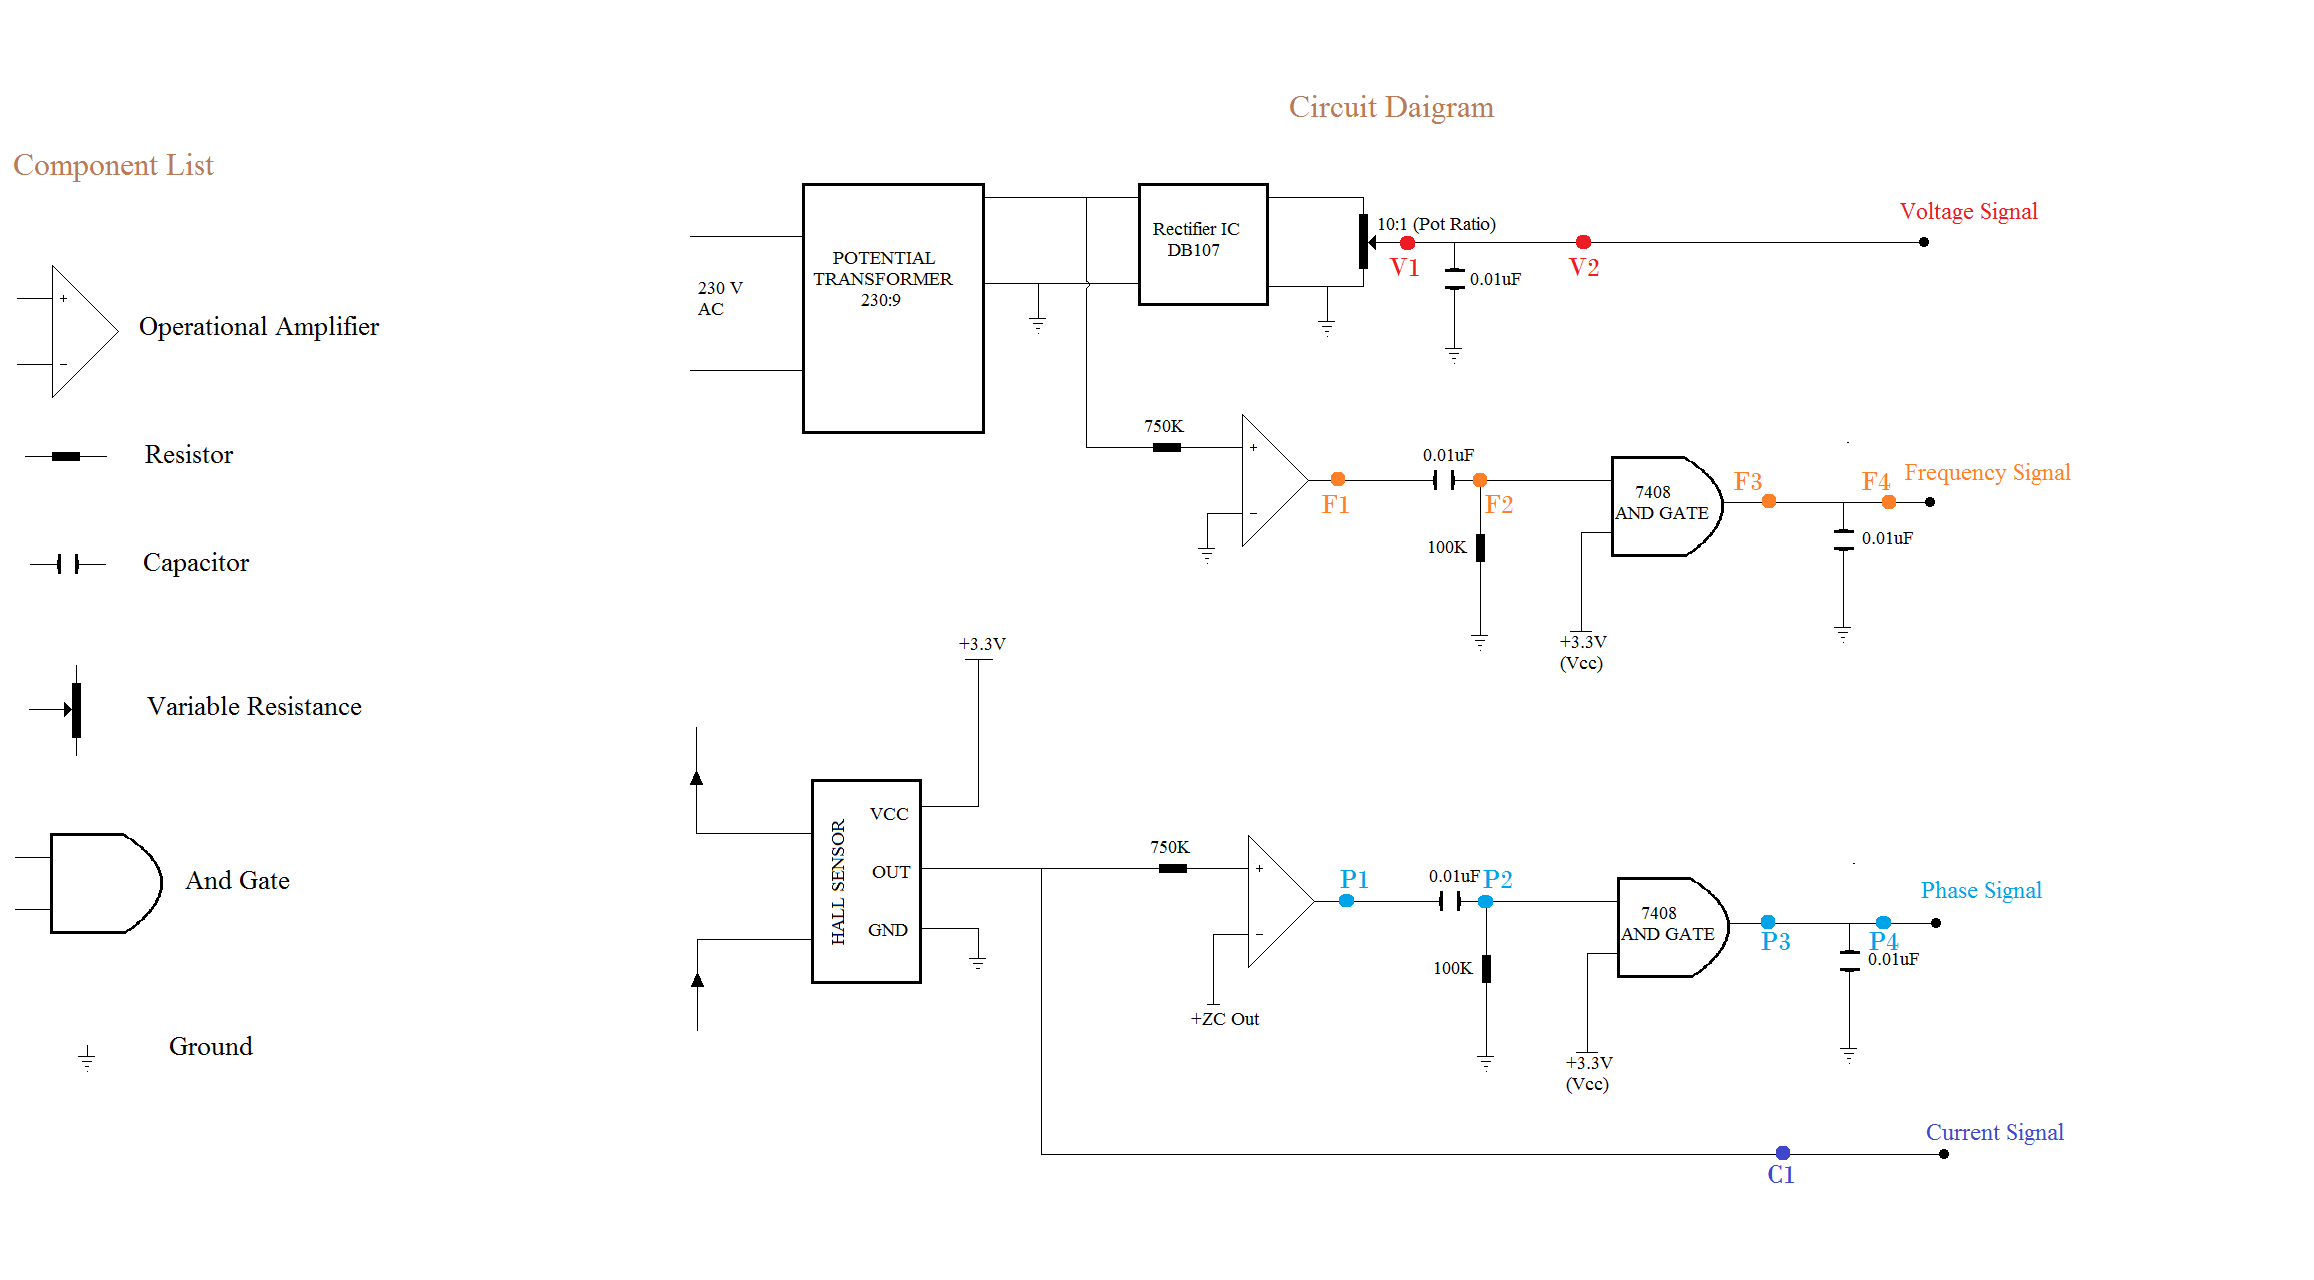
\includegraphics[width=300px]{circuit}
		\end{figure}
	\end{itemize}
\end{frame}

\begin{frame}{Task Accomplised}
	\begin{itemize}
		\item Circuit of voltage measurement has been designed and tested. 
		\item Current measurement circuit has been designed using \textbf{Hall Sensor} but will test in further weeks.
		\item Observations are as follows:-
		\vspace{0.3cm}
		\begin{figure}[h]
			\hspace{-1.25cm}
			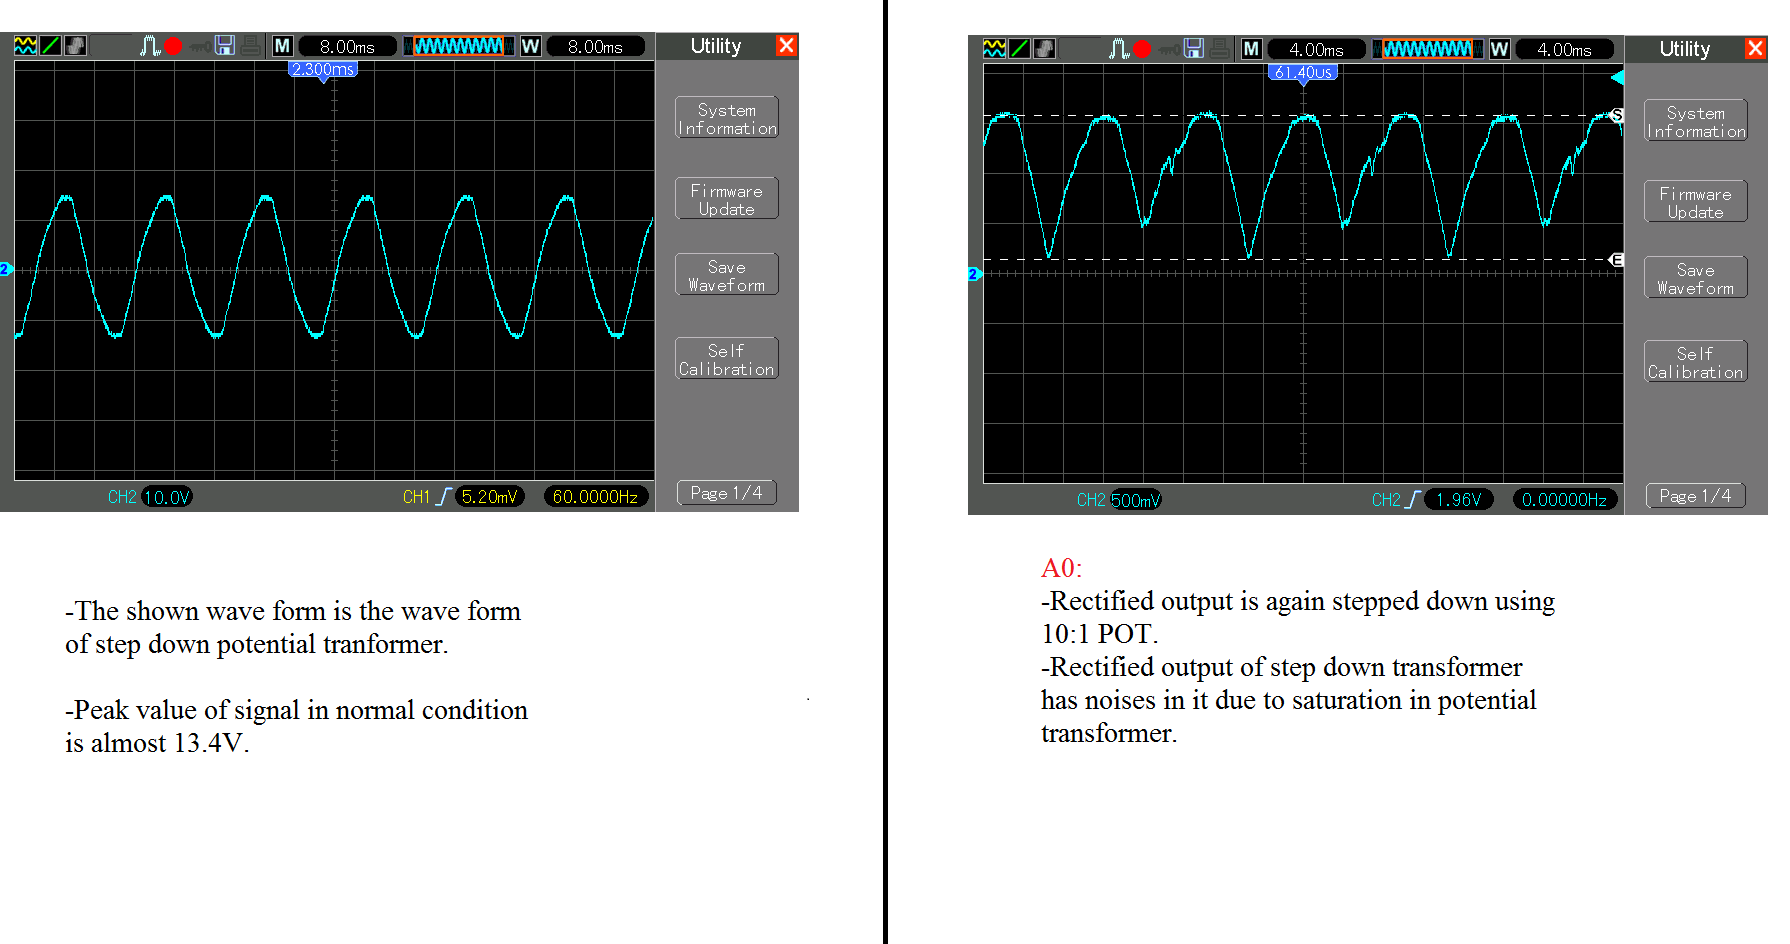
\includegraphics[width=300px]{voltage_circuit}
		\end{figure}
	\end{itemize}
\end{frame}
\begin{frame}{Task Accomplised}
		\begin{figure}[h]
			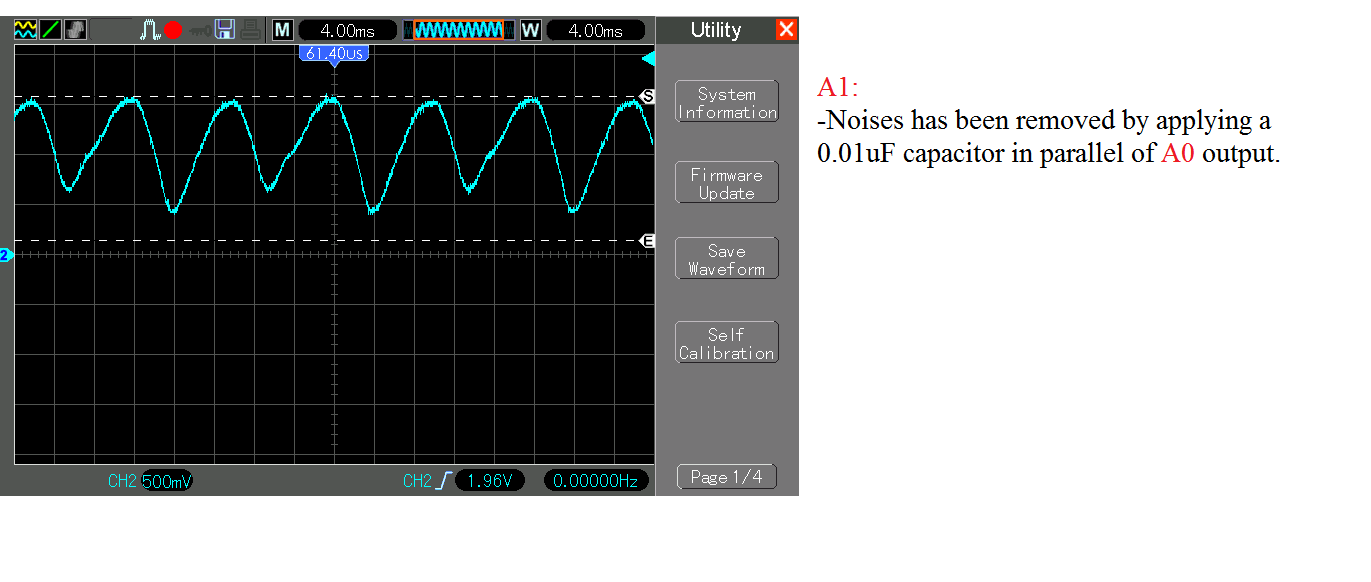
\includegraphics[width=300px]{voltage1}
		\end{figure}
\end{frame}

\begin{frame}{Task Accomplised}
	\begin{itemize}
		\item Circuit of frequency and phase measurement has been designed and tested for different load condition. 
		\begin{enumerate}
			\item Frequency measurement circuit observations are as follows:-
			 \begin{figure}[h]
			 	\hspace{-2cm}
			 	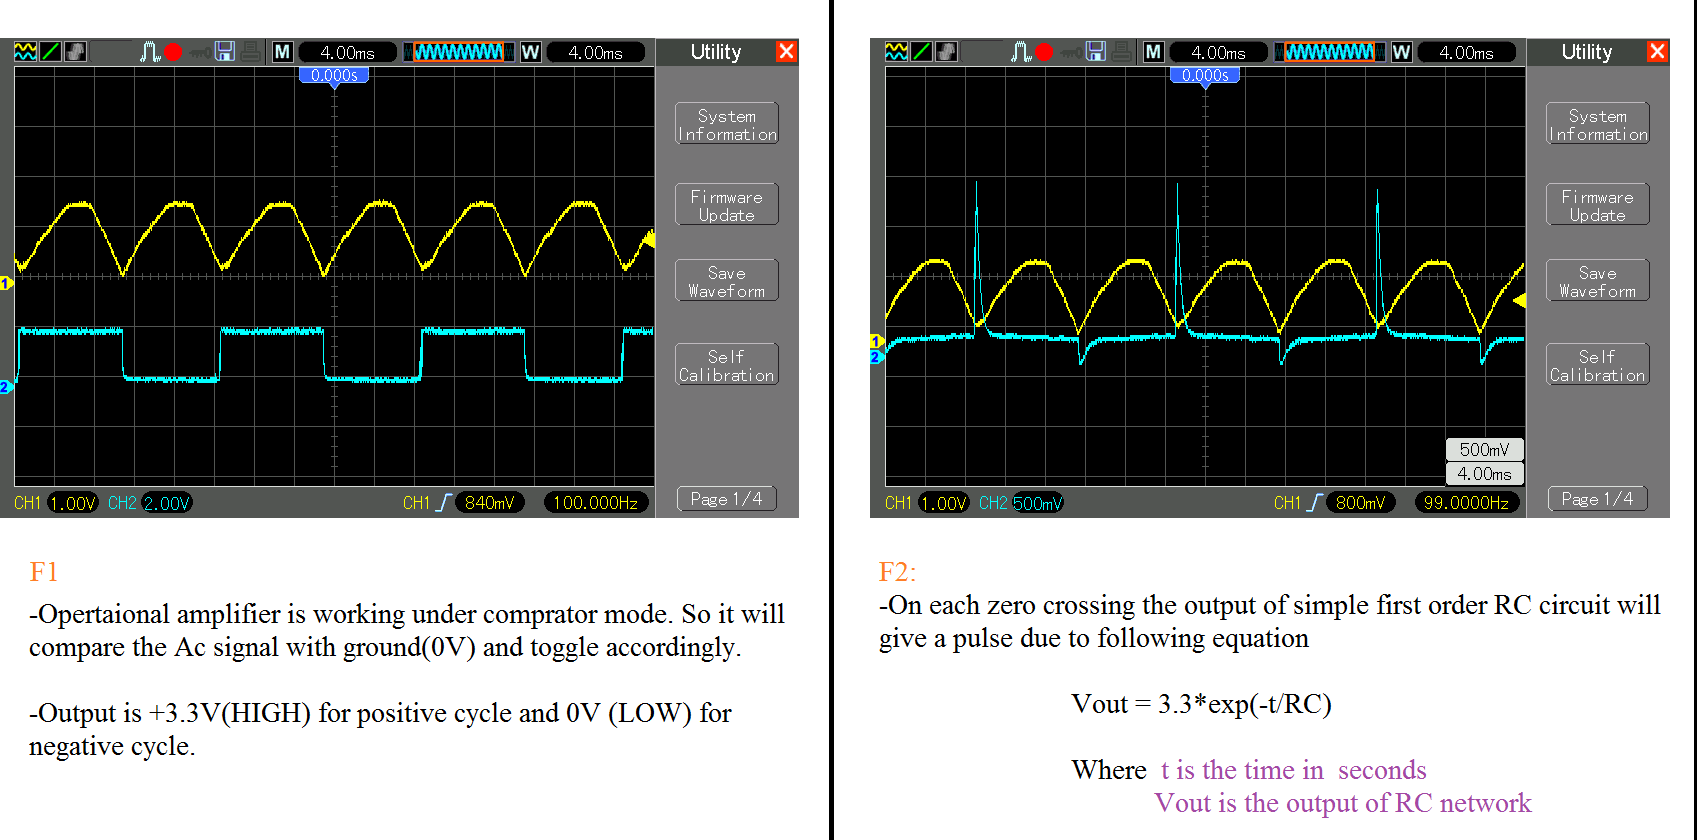
\includegraphics[width=300px]{freq_circuit1}
			 \end{figure}
		\end{enumerate}
	\end{itemize}
\end{frame}
\begin{frame}{Task Accomplised}
	\begin{figure}[h]
		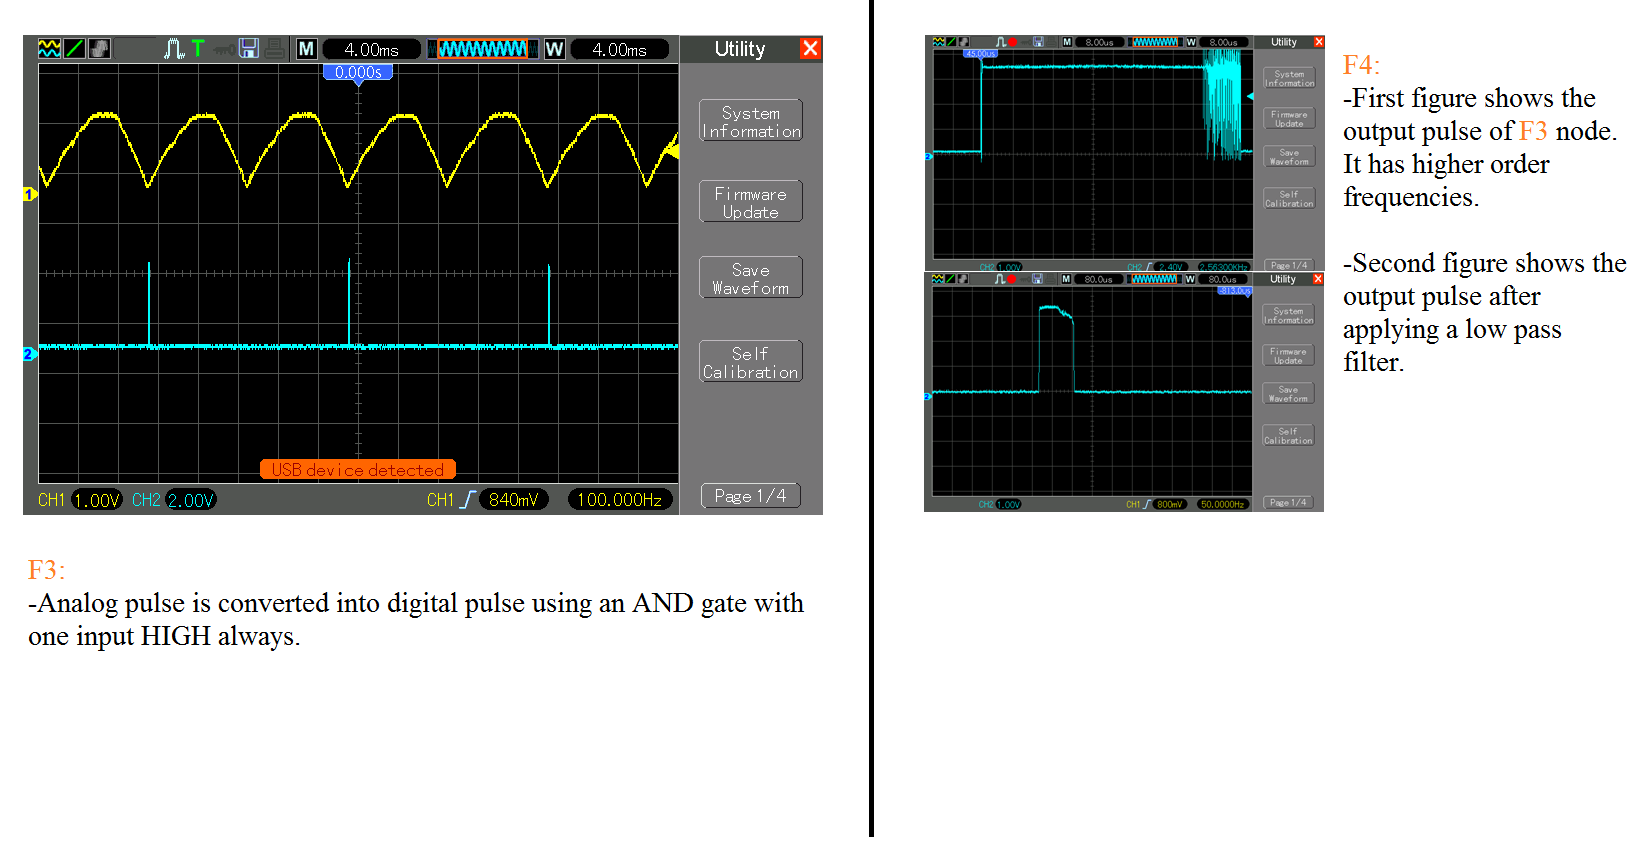
\includegraphics[width=300px]{freq_circuit2}
	\end{figure}
\end{frame}

\begin{frame}{Task Accomplised}
	\begin{itemize}
		\item Phase measurement circuit observation are as follows:-  
		\begin{figure}[h]
			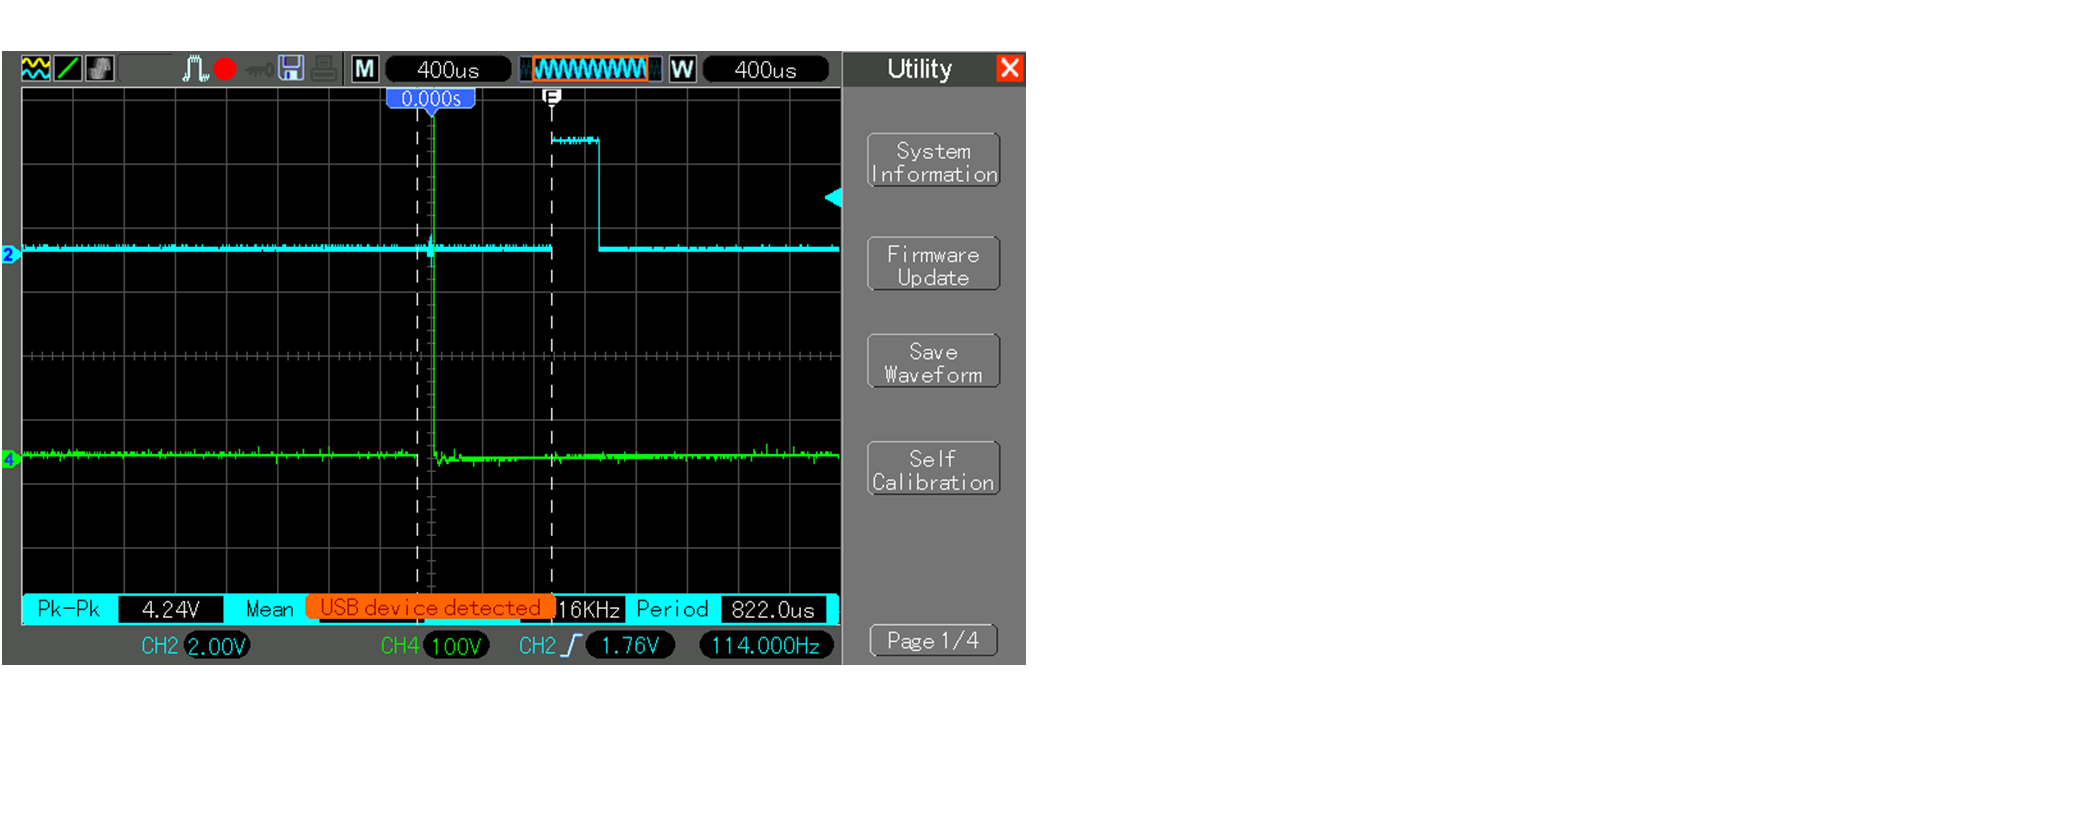
\includegraphics[width=300px]{phase_circuit}
		\end{figure}
	\end{itemize}
\end{frame}

\begin{frame}{Task Accomplised}
	\begin{figure}[h]
		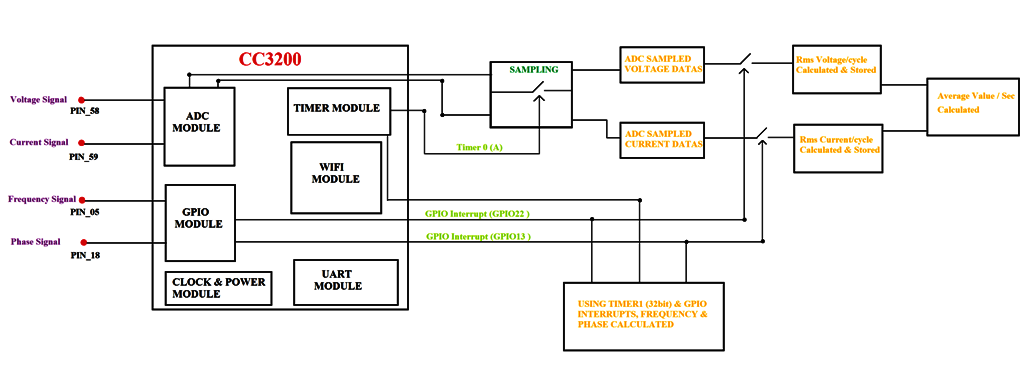
\includegraphics[width=300px]{block}
	\end{figure}
\end{frame}

\begin{frame}{Task Accomplised}
	\begin{figure}[h]
		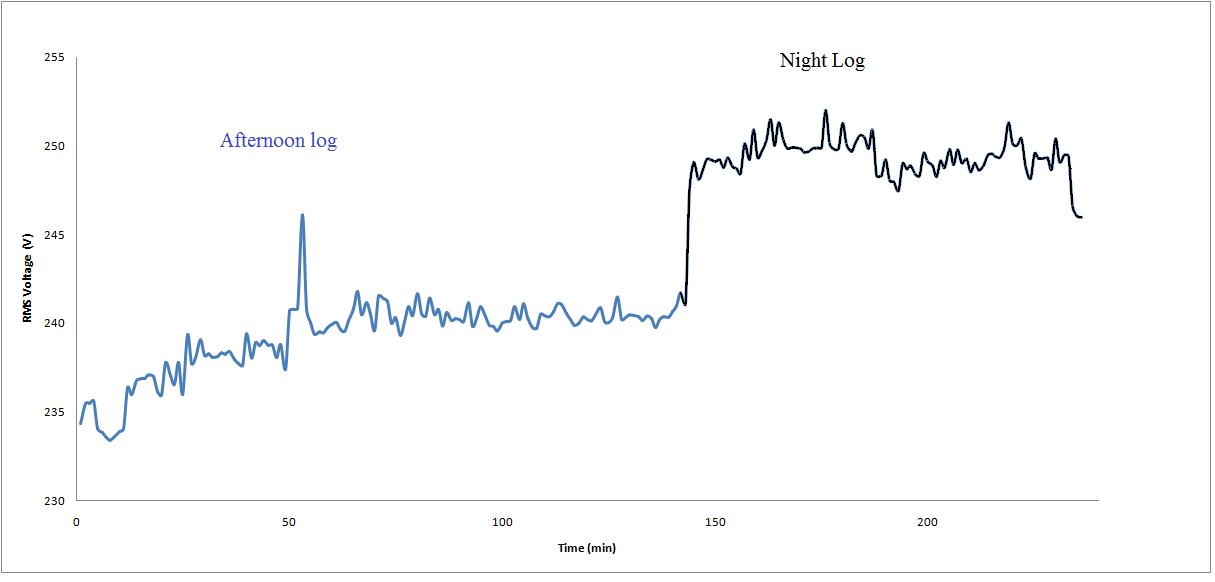
\includegraphics[width=300px]{datalog_volt}
	\end{figure}
\end{frame}


\begin{frame}{Task Accomplised}
	\begin{itemize}
		\item Web user interface and web data base has been designed and tested. But till now web page has not been linked with wifi enabled device.
		\item Snapshot of Home page is as follows:-  
		\begin{figure}[h]
			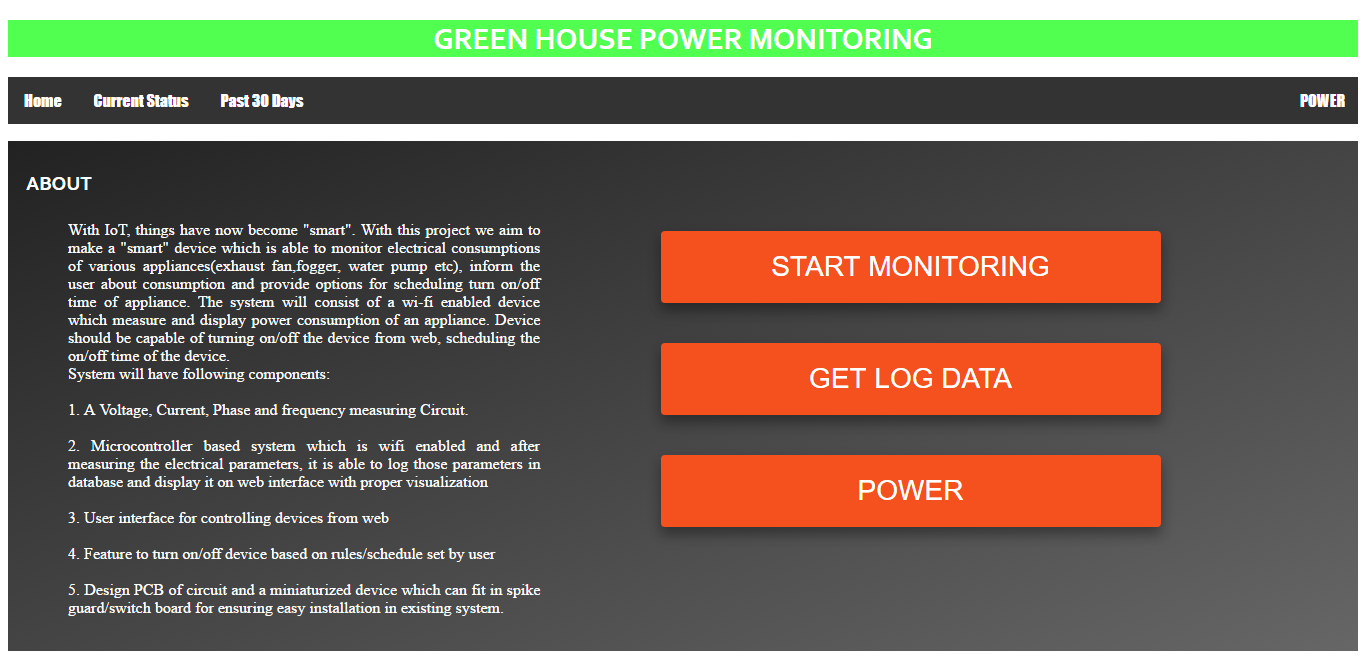
\includegraphics[width=250px]{page1}
		\end{figure}
	\end{itemize}
\end{frame}
\begin{frame}{Task Accomplised}
	\begin{itemize}
		\item Snapshot of monitoring pages are as follows:-  
		\begin{figure}[h]
			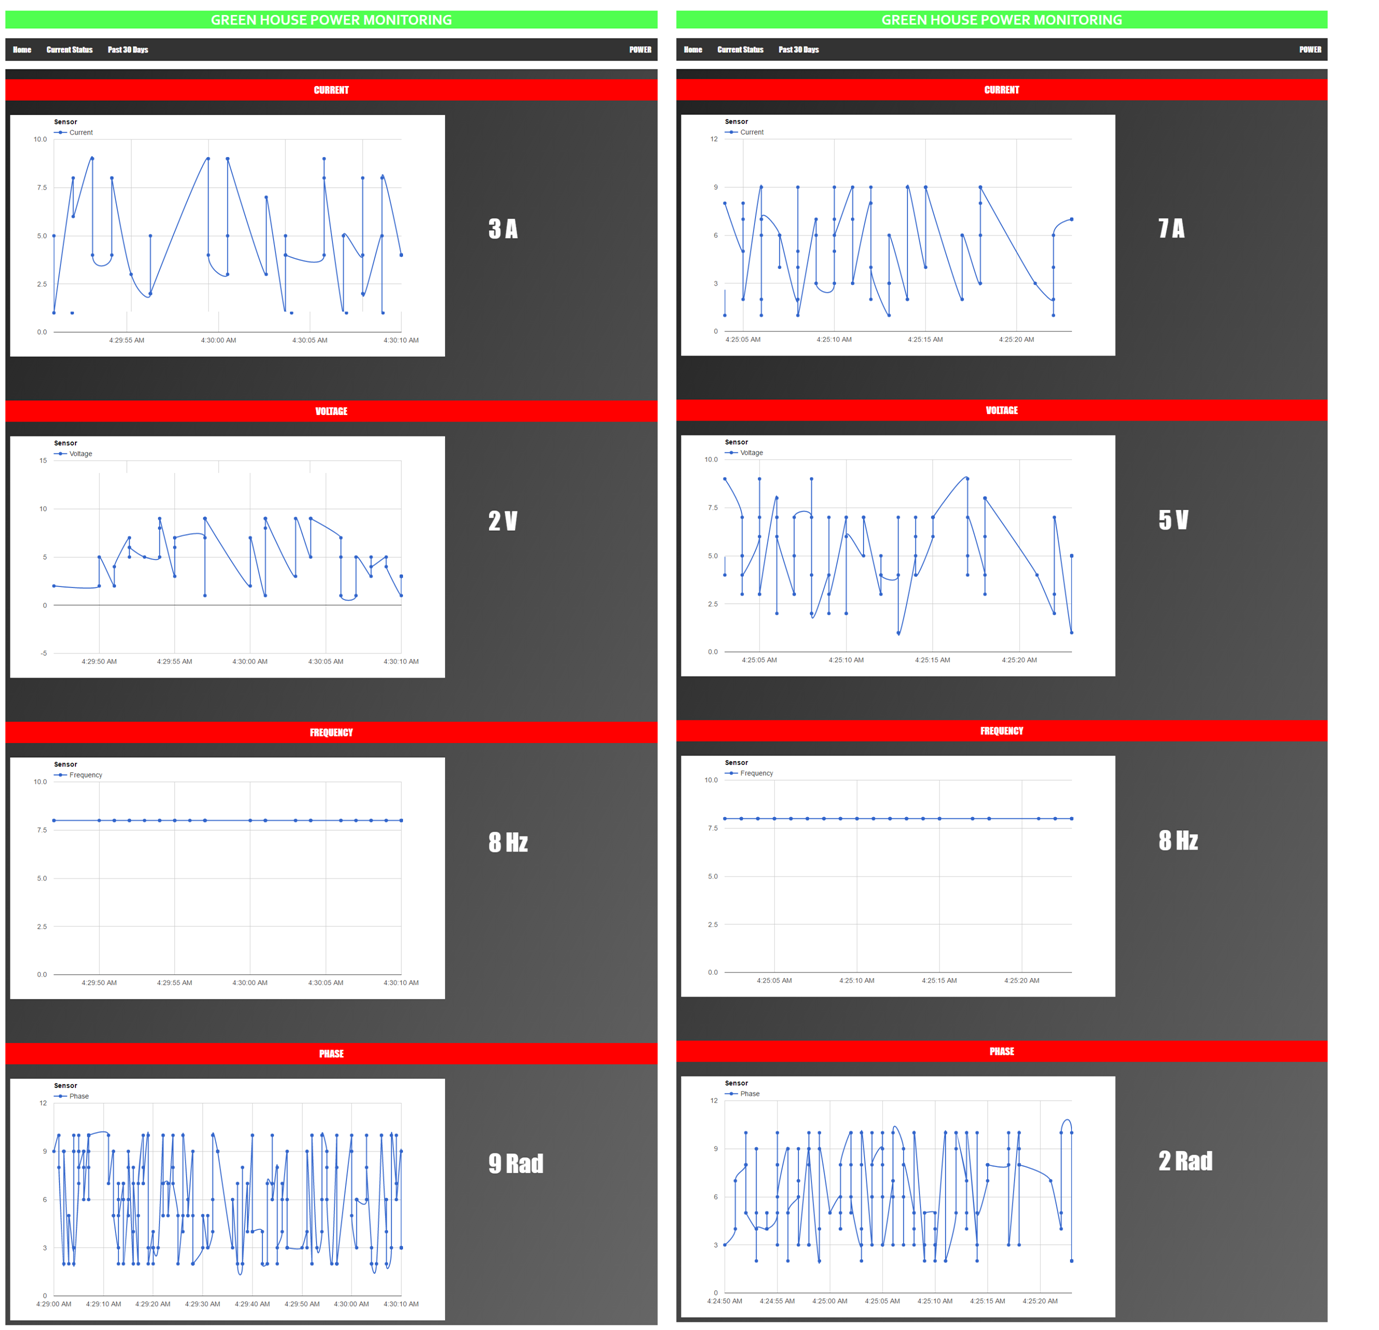
\includegraphics[width=200px]{page2}
		\end{figure}
	\end{itemize}
\end{frame}



\section{Challenges Faced}
\begin{frame}{Challenges Faced}
	\begin{itemize}
		\item Noises arrived in the measurement circuit due to saturation of Potential Transformer.
		\item Learning of CC3200 microcontroller and launchpad.
		\item Learning of Code Composer Studio.
		\item Real Time Updating Graphs.
		\item Sending Data to Database Using CC3200 wifi launchpad.    
	\end{itemize}
\end{frame}

\section{Future Plans}
\begin{frame}{Future Plans}
	\begin{itemize}
		\item Setting up a relay in device for remote controlling.
		\item Logging data in database using CC3200 launchpad.
		\item PCB designing and creating a miniature version of device so that it can easily fit in a plug hence a \textbf{"Smart plug"}.
		\item Concentrating on power management of device using CC3200 inbuilt power features like Hibernate mode,sleep mode etc.   
	\end{itemize}
\end{frame}

\section{References}
\begin{frame}{References}
	\begin{itemize}
	\item \url{stackoverflow.com}
	\item \url{developers.google.com/chart}
	\item \url{e2e.ti.com}
	\item \url{arduinosensors.com/index.php/tag/allegro-acs712} 
	\end{itemize}
\end{frame}
\section{Thank You}
\begin{frame}{Thank You}
	\centering THANK YOU !!!
\end{frame}
\end{document}
